\documentclass{beamer}
\usefonttheme[onlymath]{serif}
\usepackage[T1]{fontenc}
\usepackage[utf8]{inputenc}
\usepackage[english, icelandic]{babel}
\usepackage{amsmath}
\usepackage{amssymb}
\usepackage{amsthm}
\usepackage{gensymb}
\usepackage{parskip}
\usepackage{mathtools}
\usepackage{listings}
\usepackage{xfrac}
\usepackage{graphicx}
\usepackage{xcolor}
\usepackage{tikz}
\usetikzlibrary{calc}
\usepackage{multicol}

\DeclareMathOperator{\lcm}{lcm}
\DeclareMathOperator{\diam}{diam}
\DeclareMathOperator{\dist}{dist}
\DeclareMathOperator{\ord}{ord}
\DeclareMathOperator{\Aut}{Aut}
\DeclareMathOperator{\Inn}{Inn}
\DeclareMathOperator{\Ker}{Ker}
\DeclareMathOperator{\trace}{trace}
\DeclareMathOperator{\fix}{fix}
\DeclareMathOperator{\Log}{Log}
\renewcommand\O{\mathcal{O}}
\newcommand\floor[1]{\left\lfloor#1\right\rfloor}
\newcommand\ceil[1]{\left\lceil#1\right\rceil}
\newcommand\abs[1]{\left|#1\right|}
\newcommand\p[1]{\left(#1\right)}
\newcommand\sqp[1]{\left[#1\right]}
\newcommand\cp[1]{\left\{#1\right\}}
\newcommand\norm[1]{\left\lVert#1\right\rVert}
\renewcommand\qedsymbol{$\blacksquare$}
\renewcommand\Im{\operatorname{Im}}
\renewcommand\Re{\operatorname{Re}}
\usepackage{color}

\definecolor{mygray}{rgb}{0.4,0.4,0.4}
\definecolor{mygreen}{rgb}{0, 0, 1}
\definecolor{myorange}{rgb}{1.0,0.4,0}

\lstset{
commentstyle=\color{mygray},
numbersep=5pt,
numberstyle=\tiny\color{mygray},
keywordstyle=\color{mygreen},
showspaces=false,
showstringspaces=false,
stringstyle=\color{myorange},
tabsize=4
}
\lstset{literate=
{æ}{{\ae}}1
{í}{{\'{i}}}1
{ó}{{\'{o}}}1
{á}{{\'{a}}}1
{é}{{\'{e}}}1
{ú}{{\'{u}}}1
{ý}{{\'{y}}}1
{ð}{{\dh}}1
{þ}{{\th}}1
{ö}{{\"o}}1
{Á}{{\'{A}}}1
{Í}{{\'{I}}}1
{Ó}{{\'{O}}}1
{Ú}{{\'{U}}}1
{Æ}{{\AE}}1
{Ö}{{\"O}}1
{Ø}{{\O}}1
{Þ}{{\TH}}1
}

\usetheme{Madrid}

\title{Gagnagrindur}
\subtitle{Rótarþáttun, Fenwick-tré og fylkjaaðgerðir}
\author{Bergur Snorrason}
\date{\today}

\AtBeginSection[] {
  \begin{frame}
    \frametitle{Efnisyfirlit}
    \tableofcontents[currentsection]
  \end{frame}
}

\begin{document}

\frame{\titlepage}

\section[Miðmisseriskeppnin]{Miðmisseriskeppnin}

\begin{frame}
	\frametitle{Keppnin}
\begin{itemize}
	\item<1-> Miðmisseriskeppnin verður haldin í næstu viku.
	\item<2-> Í keppninni verða sex dæmi.
	\item<3-> Keppnin hefst $15:00$ og lýkur $18:00$.
	\item<4-> Keppnin kemur í stað dæmaskila þá vikuna.
\end{itemize}
\end{frame}

\section[Inngangur]{Inngangur}

\begin{frame}
	\frametitle{Dæmi þannig að varla þarf á öðrum dæmi að halda}
\begin{itemize}
	\item<1-> Fyrsta lína inntaksins inniheldur tvær heiltölur $n$ og $m$.
	\item<2-> Næsta lína innheldur lista af $n$ helitölum.
	\item<3-> Næstu $m$ línur verða af tveimur gerðum:
		\begin{itemize}
			\item<4-> \texttt{1 q p} þýðir að breyta eigi $p$-ta staki listans í $q$.
			\item<5-> \texttt{2 q p} þýðir að prenta eigi summu stakanna í $q$-ta til $p$-ta sæti.
		\end{itemize}
\end{itemize}
\end{frame}

\begin{frame}[fragile]
	\frametitle{Dæmi þannig að varla þarf á öðrum dæmi að halda}
\begin{itemize}
	\item<1-> Rennum í gegnum eitt sýnidæmi. Látum inntakið vera
		\item<2->\begin{verbatim}
		10 6
		0 1 2 3 4 5 6 7 8 9
		2 0 9
		2 0 4
		1 2 4
		1 6 0
		1 7 1
		2 1 8
		\end{verbatim}
\end{itemize}
\end{frame}

\begin{frame}
	\frametitle{Dæmi þannig að varla þarf á öðrum dæmi að halda}
\begin{itemize}
	\item<1-> Fylkið byrjar sem $[0\ 1\ 2\ 3\ 4\ 5\ 6\ 7\ 8\ 9]$.
	\item<2-> Eftir \texttt{2 0 9} á að skila $0 + 1 + 2 + 3 + 4 + 5 + 6 + 7 + 8 + 9 = 45$.
	\item<3-> Eftir \texttt{2 0 4} á að skila $0 + 1 + 2 + 3 + 4 = 10$.
	\item<4-> Eftir \texttt{1 2 4} verður fylkið $[0\ 1\ 4\ 3\ 4\ 5\ 6\ 7\ 8\ 9]$.
	\item<5-> Eftir \texttt{1 6 0} verður fylkið $[0\ 1\ 4\ 3\ 4\ 5\ 0\ 7\ 8\ 9]$.
	\item<6-> Eftir \texttt{1 7 1} verður fylkið $[0\ 1\ 4\ 3\ 4\ 5\ 0\ 1\ 8\ 9]$.
	\item<7-> Eftir \texttt{2 1 8} á að skila $1 + 4 + 3 + 4 + 5 + 0 + 1 + 8 = 26$.
\end{itemize}
\end{frame}

\begin{frame}
	\frametitle{Frumstæð lausn}
\begin{itemize}
	\item<1-> Það liggur helst við að leysa þetta línulega.
	\item<2-> Við látum allar tölurnar í $n$ staka fylki.
	\item<3-> Fyrir fyrri aðgerðina breytum við tilheyrandi staki í fylkinu.
	\item<4-> Fyrir seinni aðgerðina löbbum við í gegnum fylkið og reiknum summuna.
	\item<5-> Fyrri aðgerðin er $\O(1)$ og seinni aðgerðin er $\O(n)$,
		svo tímaflækjan er $\O(nm)$.
\end{itemize}
\end{frame}

\section[Rótarþáttun]{Rótarþáttun}

\begin{frame}
	\frametitle{Almenn $k$-þáttun}
\begin{itemize}
	\item<1-> Hvað ef við skiptum fylkinu upp í $k$ hólf.
	\item<2-> Við getum þá haldið utan um, og uppfært, summu hvers hólfs auðveldlega.
	\item<3-> Til að finna summu á einhverju bili í fylkinu nægir að reikna summu hólfana á milli
		endapunktana og leggja svo afganginn við (afgangurinn er í mesta lagi lengd tveggja hólfa).
	\item<4-> Ef við skiptum fylkinu úr sýnidæminu upp í $3$ hólf þá verður það
		\[
			p = [0\ 1\ 4\ |\ 3\ 4\ 5\ |\ 0\ 1\ 8\ 9].
		\]
	\item<5-> Köllum fylkið sem geymir summu hvers hólfs $s$. Það verður nú
		\[
			s = [5\ 12\ 18].
		\]
\end{itemize}
\end{frame}

\begin{frame}
	\frametitle{Fyrri aðgerð með almennri $k$-þáttun}
\begin{itemize}
	\item<1-> Ef við viljum uppfæra, til dæmis breyta staki $2$ í $9$ þá þurfum við að sjálfsögðu að uppfæra
		$p$, en það þarf líka breyta $s$.
	\item<2-> Til að breyta $p$ gerum við einfaldlega \texttt{p[2] = 9}.
	\item<3-> Til að uppfæra $s$ þurfum við að finna hólfið sem stak $2$ tilheyrir. Þar sem það er í hólfi $0$
		notum við \texttt{s[0] = s[0] - p[2] + 9}.
	\item<4-> Glöggir lesendur taka þó eftir að við þurfum að uppfæra $s$ {\bf áður} en við uppfærum $p$, þar sem
		við notum gamla gildi $p$ þegar við uppfærum $s$.
	\item<5-> Svona líta svo fylkin út, fyrir og eftir uppfærslu.
		\[
		\begin {array}{c c}
		\text{Fyrir breytingu} & \text{Eftir breytingu}\\
			p = [0\ 1\ 4\ |\ 3\ 4\ 5\ |\ 0\ 1\ 8\ 9] & p = [0\ 1\ 9\ |\ 3\ 4\ 5\ |\ 0\ 1\ 8\ 9]\\
			s = [5\ 12\ 18] & s = [10\ 12\ 18]
		\end {array}.
		\]
\end{itemize}
\end{frame}

\begin{frame}
	\frametitle{Seinni aðgerðin með almennri $k$-þáttun}
\begin{itemize}
	\item<1-> Ég fór mjög losaralega í hvernig ætti að framkalla seinni aðgerðina.
	\item<2-> Skoðum, sem dæmi, hverju eigi að skila fyrir \texttt{2 1 8}.
	\item<3-> Það er aðeins eitt hólf á milli staks $1$ og staks $8$, hólf $1$.
	\item<4-> "Afgangurinn", eins og ég kallaði það áðan, eru þau stök sem ekki eru í hólfi $1$
		en eru þó á bilinu frá $1$ til $8$.
	\item<5-> Þetta eru stök $1$, $2$, $6$, $7$ og $8$ (samtals summan er þá $31$).
	\item<6-> Við erum því að leggja saman rauðu stökin á myndinni fyrir neðan.
		\[
		\begin {array}{c}
			p = [0\ {\color{red} 1 \ 9\ }|\ {\color{blue}3\ 4\ 5\ } |\ {\color{red} 0\ 1\ 8\ } 9]\\ 
			s = [10\ \alert{12}\ 18]
		\end {array}.
		\]
	\item<7-> Þið getið ímyndað ykkur hvað við getum sparað mikinn tíma fyrir stærri fylki (sem
		við skiptum upp í fleiri hólf).
\end{itemize}
\end{frame}

\begin{frame}
	\frametitle{Tímflækja almennar $k$-þáttunar}
\begin{itemize}
	\item<1-> En er þetta hraðar en frumstæða aðferðin sem við skoðuðum í upphafi?
	\item<2-> Það fer að sjálfsögðu allt eftir því hversu stór hólf við veljum.
	\item<3-> Ef fylkinu er skipt upp í $n$ hólf er nokkuð ljóst að þessi aðferð er jafngild frumstæðu aðferðinni.
	\item<4-> Ef fylkinu er skipt upp í $1$ hólf gildir það sama.
	\item<5-> Munið að við létum $k$ tákna fjölda hólfa.
	\item<6-> Fyrri aðgerðin er ennþá $\O(1)$, en seinni aðgerðin verður $\O\left(\frac{n}{k} + k\right )$,
		svo tímaflækjan er $\O\left (\frac{mn}{k} + mk \right )$.
\end{itemize}
\end{frame}

\begin{frame}
	\frametitle{Skynsamlegt val á $k$ (Þið megið sleppa þessari glæru ef þið viljið)}
\begin{itemize}
	\item Þar sem að fyrrir aðgerðin er ekki háð skiptingunni þá nægir að lágmarka $\frac{n}{k} + k$.
	\pause\item Látum $f(k) = \frac{n}{k} + k$.
	\pause\item Við höfum $f'(k) = -\frac{n}{k^2} + 1$.
	\pause\item Útgildispunktar fást í
		\[
			\begin{array}{l l}
			\pause& f'(k) = 0\\
			\pause\Rightarrow & 1 - \frac{n}{k^2} = 0\\
			\pause\Rightarrow & 1 = \frac{n}{k^2}\\
			\pause\Rightarrow & k^2 = n\\
			\pause\Rightarrow & k = \sqrt{n}
		\end{array}
		\]
	\pause\item Nú þarf bara að ganga úr skugga um að þessi skipting sé betri en línuleg.
\end{itemize}
\end{frame}

\begin{frame}
	\frametitle{Skynsamlegt val á $k$}
\begin{itemize}
	\item Ef við veljum $k = \sqrt{n}$ þá er tímaflækja seinni aðgerðarinnar
		\pause
		\[
			\O \left (\frac{n}{\sqrt{n}} + \sqrt{n}\right ) = \O (\sqrt{n} + \sqrt{n}) = \O (\sqrt{n})
		\]
	\pause\item Því er tímaflækjan á lausninni $\O(m\sqrt{n})$.
	\pause\item Svo þessi aðferð er betri en sú frumstæða, ef við skiptum í $\sqrt{n}$ hólf.
	\pause\item Við köllum það rótarþáttun (e. squareroot decomposition) þegar við skiptum upp í $\sqrt{n}$ hólf.
\end{itemize}
\end{frame}

\section[Fenwick-tré]{Fenwick-tré}

\begin{frame}
	\frametitle{Fenwick-tré}
	\begin{itemize}
		\item<1-> Er einhver fljót leið til að reikna summu forskeyti listans?
		\item<2-> Svarið er "já, nokkrun veginn".
		\item<3-> Þetta er unnt að gera með svo kölluðum Fenwick-trjám.
		\item<4-> Skoðum fyrst nokkur atriði um framsetningu talna.
	\end{itemize}
\end{frame}

\begin{frame}
	\frametitle{Tölur í tvíundakerfi}
	\begin{itemize}
		\item<1-> Við könnumst flest við tíundaframsetningu talna, t.d.
			\[
				12045 = 1\cdot 10^4 + 2\cdot 10^3 + 0\cdot 10^2 + 4\cdot 10^1 + 5\cdot 10^0
			\]
		\item<2-> Hvað ef við notum annan veldisstofn en $10$, t.d. $2$?
		\item<3-> Það köllum við bitaframsetningu og munum tákna tölur settar fram með bitaframsetningu með $2$ í fótskrift, t.d.
			\[
				13 = 
				1\cdot 2^3 + 
				1\cdot 2^2 + 
				0\cdot 2^1 + 
				1\cdot 2^0 
				= 1101_2
			\]
		\item<4-> Stærsti biti tölunnar $b$ er fremsti ásinn í tvíundaframsetningu $b$.
		\item<5-> Minnsti biti tölunnar $b$ er aftasti ásinn í tvíundaframsetningu $b$.
	\end{itemize}
\end{frame}

\begin{frame}
	\frametitle{Skilgreining Fenwick-trjáa}
	\begin{itemize}
		\item<1-> Fenwick-tré er tré sem inniheldur lykil $k$ og gildi $x$ í hverri nóðu. Ef það eru $n$ nóður
			í trénu er $0 \leq k < n$.
		\item<2-> Nóðan með lykil $0$ er rót trésins.
		\item<3-> Nóða með lykil $k$ er barn nóðu með lykil $m$ ef og aðeins ef $k$ og $m$ hafa sömu bitaframsetningu
			fyrir utan minnsta bita $k$.
		\item<4-> ATH: Fenwick-tré eru ekki tvíundatré.
	\end{itemize}
\end{frame}

\begin{frame}
	\frametitle{Nokkur dæmi}
	\begin{itemize}
		\item<1-> Skoðum bitframsetningu talna minni en $16$.
			\small
			\[
				\begin{array}{l l}
					0 &  0000\\
					1 &  0001\\
					2 &  0010\\
					3 &  0011\\
					4 &  0100\\
					5 &  0101\\
					6 &  0110\\
					7 &  0111\\
					8 &  1000\\
					9 &  1001\\
					10 & 1010\\
					11 & 1011\\
					12 & 1100\\
					13 & 1101\\
					14 & 1110\\
					15 & 1111\\
			\end{array}
			\]
	\end{itemize}
\end{frame}

\begin{frame}
\frametitle{Mynd af Fenwick-tréi með $16$ nóður}
	\begin{figure}
		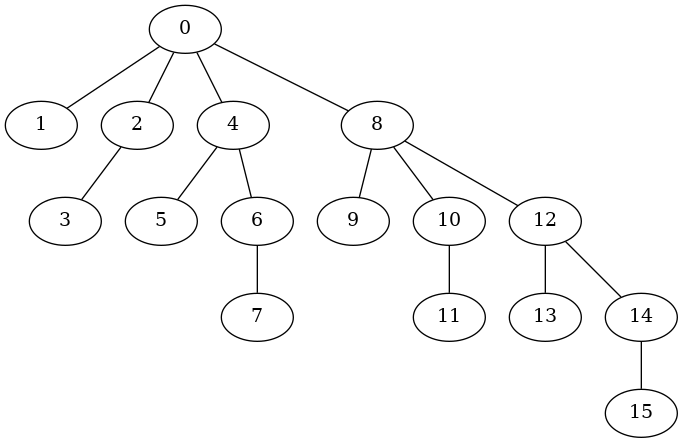
\includegraphics[scale=0.3]{mynd2.png}
	\end{figure}
\end{frame}

\begin{frame}
	\frametitle{Útfærslan á járninu}
	\begin{itemize}
		\item<1-> Þar sem að lykarnir eru einræðir og ekki stærri en $n$ þá getum við einfaldlega geymt gögnin í fylki.
		\item<2-> Nánar tiltekið, ef gildi $x$ er í nóðu með lykil $k$ látum við stak $k$ í fylkinu bera gildið $x$.
		\item<3-> Okkar vantar bara leið til að ferðast í trénu.
		\item<4-> Við munum nýta okkur að:
			\begin{itemize}
				\item<5-> Við getum dregið frá minnsta bitann til að fara upp tréð.
				\item<6-> Við getum lagt minnsta við bitann til að fara til \emph{hægri} í trénu.
			\end{itemize}
	\end{itemize}
\end{frame}

\begin{frame}
	\frametitle{Trjáa rölt}
	\begin{itemize}
		\item<1-> En hvernig hjálpar þetta okkur að leysa dæmið?
		\item<2-> Látum $p$ tákna fylkið sem geymir gögnin okkar og $f$ fylkið sem geymir tréð.
		\item<3-> Stak $i$ í $f$ geymir summmu þeirra staka frá $p[j]$ til $p[i]$, þar sem $j$ er foreldri 
			$i$ í Fenwick-trénu.
	\end{itemize}
\end{frame}

\begin{frame}[fragile]
	\frametitle{Að finna summu fyrstu $i$ stakanna}
	\begin{itemize}
		\item<1-> Til að finna summu fyrstu $i$ stakanna getum lagt saman þau stök í trénu sem svara til ásanna í bitaframsetningu $i$.
		\item<2-> Tökum sem dæmi $i = 11$. Við vitum að $11 = 1011_2$ svo stökin sem við höfum áhuga á eru $1011_2 = 11$, $1010_2 = 10$
			og $1000_2 = 8$.
		\item<3-> Summa þessara þriggja staka í trénu er þá summu fyrstu $11$ stakanna í fylkinu.
		\item<4-> Takið eftir að til fá tölurnar drögum við ítrekað frá minnsta bita tölunnar í hvert skipti. Svo útfært er fallið
		\tiny
		\begin{lstlisting}[language=C]
#define LSB(i) ((i) & -(i))

int sum(int i)
{
	int sum = 0;
	while (i > 0) 
	{
		sum = sum + a[i];
		i = i - LSB(i);
	}
	return sum;
}
\end{lstlisting}
	\end{itemize}
\end{frame}

\begin{frame}[fragile]
	\frametitle{Að uppfæra stak $i$}
	\begin{itemize}
		\item<1-> Það nægir ekki að uppfæra stak $i$ í trénu.
		\item<2-> Tökum aftur sem dæmi $11$. Þá þurfum við að uppfæra $1011_2 = 11$, $1100_2 = 12$ og $10000_2 = 16$.
		\item<3-> Núna erum við að leggja minnsta bitann við tölunna í hvert skipti.
		\item<4-> Við þyrftum svo einnig að leggja við öll önnur veldi af $2$ hærri en $16$ og minni eða jöfn heildarstærðinni.
		\item<5-> Útfært er þetta
		\tiny
		\begin{lstlisting}[language=C]
#define LSB(i) ((i) & -(i))

void add(int i, int k)
{
	while (i < n) 
	{
		a[i] = a[i] + k;
		i = i + LSB(i);
	}
}
		\end{lstlisting}
	\end{itemize}
\end{frame}

\begin{frame}
	\frametitle{Niðurstaða}
	\begin{itemize}
		\item<1-> Fenwick-tré styðja ekki beint leitir að hlutbilssummum á forminu $[a, b]$.
		\item<2-> Við getum þó reiknað hlutbilssummur $[0, a - 1]$ og $[0, b]$ og mismunur þeirra gefur hlutbilssummu $[a, b]$.
		\item<3-> Við getum nú uppfært og reiknað hlutbilssummur í $\O(\log n)$, sem er betra en rótarþáttunin.
	\end{itemize}
\end{frame}

\section[Fylkjaaðgerðir]{Fylkjaaðgerðir}

\begin{frame}
	\frametitle{Fylki í stærðfræði}
	\begin{itemize}
		\item<1-> \emph{Fylki} í stærðfræði er annað en \emph{fylki} í tölvunarfræði.
		\item<2-> Í stærðfræði eru fylki eins og tvívíð tölvunarfræði-fylki.
		\item<3-> Við segjum að fylki sé $a \times b$ (lesið "$a$ sinnum $b$") ef það hefur $a$ línur og $b$ dálka.
		\item<4-> Dæmi um fylki er
			\[
				\left (
				\begin{array}{c c c}
					1 & 0 & 1\\
					0 & 1 & 0
				\end{array}
				\right )
				\text{ eða }
				\left [
				\begin{array}{c c c}
					1 & 0 & 1\\
					0 & 1 & 0
				\end{array}
				\right ]
			\]
		\item<5-> Þetta fylki er $2 \times 3$.
	\end{itemize}
\end{frame}

\begin{frame}
	\frametitle{Frægustu fylkin}
	\begin{itemize}
		\item<1-> Mikilvægasta flykið sem við rekumst á er \emph{einingarfylkið}
			\[
				I :=
				\left (
				\begin{array}{c c}
					1 & 0\\
					0 & 1
				\end{array}
				\right )
			\]
		\item<2-> Annað fylki sem mun mögulega nýtast ykkur seinna meira er \emph{snúnigsfylkið}
			\[
			\sigma(\theta) =
				\left (
				\begin{array}{c c}
					\cos \theta & -\sin \theta\\
					\sin \theta & \cos \theta
				\end{array}
				\right )
			\]
	\end{itemize}
\end{frame}

\begin{frame}
	\frametitle{Skölun og samlagning}
	\begin{itemize}
		\item<1-> Ef $a$ er rauntala og $A$ er fylki, þá látum við $aA$ vera fylkið sem er eins og $A$ nema að $a$ hefur verið
			margfaldið við sérhvert stak.
		\item<2-> Ef $A$ og $B$ eru fylki sem eru bæði $a \times b$ þá getum við lagt þau saman. Summan $A + B$ er stakvís samlagning
			fylkjanna $A$ og $B$.
	\end{itemize}
\end{frame}

\begin{frame}[fragile]
	\frametitle{Fylkjasamlagning í \texttt{C}}
\begin{lstlisting}[language=C]
for (i = 0; i < a; i++)
{
	for (j = 0; j < b; j++)
	{
		r[i][j] = s[i][j] + t[i][j];
	}
}
\end{lstlisting}
\end{frame}

\begin{frame}
	\frametitle{Innfeldi}
	\begin{itemize}
		\item<1-> Ef fylkið er $1 \times n$ ($n \times 1$) þá köllum við það \emph{línuvigur} (\emph{dálkvigur}) af vídd $n$.
		\item<2-> Ef $a = (a_1, a_2, ..., a_n)$ er línuvigur og $b = (b_1, b_2, ..., b_n)$ er dálkvigur þá köllum við
			\[
				\sum_{i = 1}^{n}a_ib_i = a_1b_1 + a_2b_2 + ... + a_nb_n
			\]
		\emph{innfeldi} vigranna og táknum það $a \cdot b$.
	\end{itemize}
\end{frame}

\begin{frame}
	\frametitle{Margfeldi}
	\begin{itemize}
		\item<1-> Ef $A$ er $a \times b$ og $B$ er $b \times c$ þá getum við skilgreint margföldun fyrir fylkin.
		\item<2-> Margfeldið $AB$ verður þá $a \times c$.
		\item<3-> Stakið í línu $i$ og dálki $j$ í $AB$ fæst með því að reikna innfeldi línu $i$ í $A$ og dálk $j$ í $B$.
		\item<4-> Nánar er
			\[
				c_{ij} = \sum_{k \geq 1}a_{ik}b_{kj}, \quad \text{þar sem $c_{ij}$ er stakið í línu $i$ og dálki $j$ í $AB$.}
			\]
		\item<5-> Dæmi um einfalda fylkjamargföldun er
			\[
				\left (
				\begin{array}{c c}
					a & b\\
					c & d
				\end{array}
				\right )
				\left (
				\begin{array}{c c}
					e & f\\
					g & h
				\end{array}
				\right )
				=
				\left (
				\begin{array}{c c}
					ae + bg & af + bh\\
					ce + dg & cf + dh
				\end{array}
				\right )
			\]
	\end{itemize}
\end{frame}

\begin{frame}[fragile]
	\frametitle{Fylkjamargföldun í \texttt{C}}
\begin{lstlisting}[language=C]
for (i = 0; i < a; i++)
{
	for (j = 0; j < c; j++)
	{
		r[i][j] = 0;
		for (k = 0; k < b; k++)
		{
			r[i][j] += s[i][k]*t[k][j];
		}
	}
}
\end{lstlisting}
\end{frame}

\begin{frame}
	\frametitle{Andhverfur}
	\begin{itemize}
		\item<1-> Ef $A$  og $B$ eru $n \times n$ og $AB = I$ þá segjum við að $B$ sé \emph{andhverfa} $A$, oft táknað $A^{-1}$.
		\item<2-> Fyrir $2 \times 2$ fylki er til auðveld lokuð formúla fyrir andhverfuna, þ.e.
			\[
				\left (
				\begin{array}{c c}
					a & b\\
					c & d
				\end{array}
				\right )^{-1}
				=
				\frac{1}{ad - bc}
				\left (
				\begin{array}{c c}
					d & -b\\
					-c & a
				\end{array}
				\right ).
			\]
		\item<3-> Ljóst er að einhver vandi verður ef $ad - bc = 0$.
		\item<4-> Ef $ad - bc = 0$ þá hefur fylkið enga andhverfu og við segjum að það sé \emph{óandhverfanlegt}.
		\item<5-> {\bf Æfing:} Gangið úr skugga um að
			\[
				\frac{1}{ad - bc}
				\left (
				\begin{array}{c c}
					a & b\\
					c & d
				\end{array}
				\right )
				\left (
				\begin{array}{c c}
					d & -b\\
					-c & a
				\end{array}
				\right )
				=
				\left (
				\begin{array}{c c}
					1 & 0\\
					0 & 1
				\end{array}
				\right ).
			\]
	\end{itemize}
\end{frame}

\begin{frame}
	\frametitle{Lausnir línulegra kerfa}
	\begin{itemize}
		\item<1-> Fylki koma að mestum notum þegar við viljum leysa línuleg jöfnuhneppi.
		\item<2-> Tökum sem dæmi hneppið
			\begin{align*}
				& x + 2y + 6z = 1\\
				& 3x + 2y + 3z = 2\\
				& 4x + 2y + z = 3
			\end{align*}
		\item<3-> Við getum einnig táknað þetta hneppi með fylkjajöfnunni
			\[
				\left (
				\begin{array}{c c c}
					1 & 2 & 6\\
					3 & 2 & 3\\
					4 & 2 & 1
				\end{array}
				\right )
				\left (
				\begin{array}{c}
					x\\
					y\\
					z
				\end{array}
				\right )
				=
				\left (
				\begin{array}{c}
					1\\
					2\\
					3
				\end{array}
				\right )
			\]
	\end{itemize}
\end{frame}

\begin{frame}
	\frametitle{Línuaðgerðir}
	\begin{itemize}
		\item<1-> Kynnum nú einn örlítið breyttan rithátt. Í stað fylkjajöfnunnar á glærunni hér á undann skrifum við stundum
			\[
				\left (
				\begin{array}{c c c | c}
					1 & 2 & 6 & 1\\
					3 & 2 & 3 & 2\\
					4 & 2 & 1 & 3
				\end{array}
				\right ).
			\]
			Við köllum þetta fylki \emph{aukið}.
		\item<2-> Við munum nú skilgreina þrjár \emph{línuaðgerðir} á fylki.
			\begin{itemize}
				\item<3-> Skölun línu með fasta (sem er ekki $0$). $(L_1)$
				\item<4-> Leggja eina línu við aðra línu. $(L_2)$
				\item<5-> Skipta á tveimur línum. $(L_3)$
			\end{itemize}
		\item<6-> Lykilatriðið er að línuaðgerðirnar okkar breyta ekki línulega kerfinu okkar.
	\end{itemize}
\end{frame}

\begin{frame}
	\frametitle{Að leysa línuleg kerfi}
	\begin{itemize}
		\item Sjáum nú hvernig við getum beytt þessum línuaðgerðum til þess að leysa jöfnuhneppið okkar:
			\[
				\pause
				\left (
				\begin{array}{c c c | c}
					1 & 2 & 6 & 1\\
					3 & 2 & 3 & 2\\
					4 & 2 & 1 & 3
				\end{array}
				\right )
				\pause
				\stackrel{L_2}{\sim}
				\left (
				\begin{array}{c c c | c}
					1 & 2 & 6 & 1\\
					0 & -4 & -15 & -1\\
					4 & 2 & 1 & 3
				\end{array}
				\right )
				\pause
				\stackrel{L_2}{\sim}
				\left (
				\begin{array}{c c c | c}
					1 & 2 & 6 & 1\\
					0 & 4 & 15 & 1\\
					0 & 6 & 23 & 1
				\end{array}
				\right )
			\]
			\[
				\pause
				\stackrel{L_1}{\sim}
				\left (
				\begin{array}{c c c | c}
					2 & 4 & 12 & 2\\
					0 & 4 & 15 & 1\\
					0 & 6 & 23 & 1
				\end{array}
				\right )
				\pause
				\stackrel{L_2}{\sim}
				\left (
				\begin{array}{c c c | c}
					2 & 0 & -3 & 1\\
					0 & 4 & 15 & 1\\
					0 & 0 & 1 & -1
				\end{array}
				\right )
				\pause
				\stackrel{L_2}{\sim}
				\left (
				\begin{array}{c c c | c}
					2 & 0 & -3 & 1\\
					0 & 4 & 0 & 16\\
					0 & 0 & 1 & -1
				\end{array}
				\right )
			\]
			\[
				\pause
				\stackrel{L_2}{\sim}
				\left (
				\begin{array}{c c c | c}
					2 & 0 & 0 & -2\\
					0 & 4 & 0 & 16\\
					0 & 0 & 1 & -1
				\end{array}
				\right )
				\pause
				\stackrel{L_1}{\sim}
				\left (
				\begin{array}{c c c | c}
					1 & 0 & 0 & -1\\
					0 & 4 & 0 & 16\\
					0 & 0 & 1 & -1
				\end{array}
				\right )
				\pause
				\stackrel{L_1}{\sim}
				\left (
				\begin{array}{c c c | c}
					1 & 0 & 0 & -1\\
					0 & 1 & 0 & 4\\
					0 & 0 & 1 & -1
				\end{array}
				\right )
			\]
		\pause\item Svo $x = -1$, $y = 4$ og $z = -1$ leysir jöfnuhneppið okkar.
	\end{itemize}
\end{frame}

\begin{frame}
	\frametitle{Gauss eyðing}
	\begin{itemize}
		\item<1-> Ferlið sem ég var að ganga í gegnum er kallað \emph{Gauss-eyðing} og er algengasta leiðin til að leysa
			jöfnuhneppi.
		\item<2-> Fyrir $n \times n$ fylki er Gauss-eyðing $\O(n^3)$.
	\end{itemize}
\end{frame}

\begin{frame}[fragile]
	\frametitle{Gauss-eðying í \texttt{C++}}
	\tiny
\begin{lstlisting}[language=C++]
#define rep(i,a,b) for (__typeof(a) i=(a); i<(b); ++i)
const double EPS = 1e-9;
template <class K> bool eq(K a, K b) { return a == b; }
template <> bool eq<double>(double a, double b) {
    return abs(a - b) < EPS; }
template <class T> struct matrix {
  int rows, cols, cnt; vector<T> data;
  inline T& at(int i, int j) { return data[i * cols + j]; }
  matrix(int r, int c) : rows(r), cols(c), cnt(r * c) {
    data.assign(cnt, T(0)); }
  matrix(const matrix& other) : rows(other.rows),
    cols(other.cols), cnt(other.cnt), data(other.data) { }
  T& operator()(int i, int j) { return at(i, j); }
  matrix<T> rref(T &det, int &rank) {
    matrix<T> mat(*this); det = T(1), rank = 0;
    for (int r = 0, c = 0; c < cols; c++) {
      int k = r;
      rep(i,k+1,rows) if (abs(mat(i,c)) > abs(mat(k,c))) k = i;
      if (k >= rows || eq<T>(mat(k, c), T(0))) continue;
      if (k != r) {
        det *= T(-1);
        rep(i,0,cols) swap(mat.at(k, i), mat.at(r, i));
      } det *= mat(r, r); rank++;
      T d = mat(r,c);
      rep(i,0,cols) mat(r, i) /= d;
      rep(i,0,rows) {
        T m = mat(i, c);
        if (i != r && !eq<T>(m, T(0)))
          rep(j,0,cols) mat(i, j) -= m * mat(r, j); } r++;
    } return mat; }
};
\end{lstlisting}
\end{frame}
\end{document}
